% !TeX TXS-program:bibliography = txs:///biber
% /* $Id: Presentation_FCSM2012.tex 2205 2012-01-10 05:15:02Z vilhu001 $ */
% /* $URL: https://repository.vrdc.cornell.edu/private/jma7/FCSM2012/text/Presentation/Presentation_FCSM2012.tex $ */
\documentclass[aspectratio=169]{beamer}
\usepackage{graphicx}
\usepackage{longtable}
\usepackage{acronym}
\newcommand{\mypath}{..}
% bibliography
\usepackage[authordate,backend=biber,natbib]{biblatex-chicago}
\addbibresource{\mypath/abbrev.bib}
\addbibresource{\mypath/lehdtp.bib}
\addbibresource{\mypath/others.bib}
\addbibresource{\mypath/data.bib}
\addbibresource{\mypath/data2014.bib}

% either this combo
%\usecolortheme[RGB={0,10,182}]{structure} 
%\usetheme{Pittsburgh}
%\logo{\includegraphics[height=0.6cm]{cb_solo_red}}

% or this combo
%\usecolortheme[RGB={0,10,182}]{dove} 
\usetheme{Malmoe}
\usecolortheme{dove}
\setbeamertemplate{footline}[frame number]% page numbers and using Warsaw theme%
%\setbeamertemplate{footline}[slide number]


% Uncomment the following line if you want %
%\setbeamercovered{transparent}
\setbeamercovered{invisible}
% To remove the navigation symbols from 
% the bottom of slides%
\setbeamertemplate{navigation symbols}{} 
\setbeamertemplate{background canvas}{
\includegraphics
	[width=\paperwidth]{Censustemplate-as-bg2017}}
%
%\usepackage{bm}         % For typesetting bold math (not \mathbold)
%
\title[S2014]{What's new in LEHD Snapshot S2014}
\author{Lars Vilhuber}
\institute[US Census Bureau, Cornell University]
{
Center for Economic Studies, US Census Bureau \\
Labor Dynamics Institute, Cornell University\\
\medskip
{\emph{lars.vilhuber@$\lbrace$cornell.edu,census.gov$\rbrace$}}
}
\date{\today}
% \today will show current date. 
% Alternatively, you can specify a date.
%
\begin{document}
%

\input{../acrodefs.tex}




\begin{frame}
\titlepage
\end{frame}
%
\begin{frame}
\frametitle{Disclaimer}
\begin{block}{Disclaimer}
	\small
This presentation reports the results of research and analysis undertaken by U.S. Census Bureau staff. It has undergone a Census Bureau review more limited in scope than that given to official Census Bureau publications. This document is released to inform interested parties of ongoing research and to encourage discussion of work in progress. The views expressed herein are attributable only to the author(s) and do not represent the views of the U.S. Census Bureau, its program sponsors, Cornell University, or other data providers.
\end{block}
\end{frame}



%

\section{Introduction}
\begin{frame}[fragile]
\frametitle{The LEHD Infrastructure Files (``Snapshot'')}
\begin{block}

\begin{itemize}
	\item Big-picture overview  in \citet{tp-2006-01,AbowdEtAl2009}
    \item Definining outputs:  \ac{QWI} and to some extent the \ac{LODES} data 
    \item Files are pulled from LEHD production archives, several research-related improvements are made to the files, fixing minor data inconsistencies or     updating documentation.
    \item Do not contain any information related to the disclosure limitation measures used in the \ac{QWI}
\end{itemize}
\end{block}
\nocite{RePEc:cen:wpaper:14-26,RePEc:cen:wpaper:11-43,RePEc:cen:wpaper:11-13}.
\end{frame}


\section{S2014}
\subsection{Availability}

\begin{frame}
\frametitle{Availability by MOU}
Of the 51 states and DC, as of 2017-09-08, 12 have chosen Option A:
\begin{center}
	\begin{tabular}{lp{2in}l}
Option&&	Freq\\
\hline
A	&Data available subject to CB approval and pooling&12\\
B	&Data available subject to state approval &32\\
    & of which frequently approve projects: &13\\
NA	&Other &7\\
\end{tabular}
\end{center}
\end{frame}

\subsection{Representativeness}

\begin{frame}
	\frametitle{By employment}
	\centering
	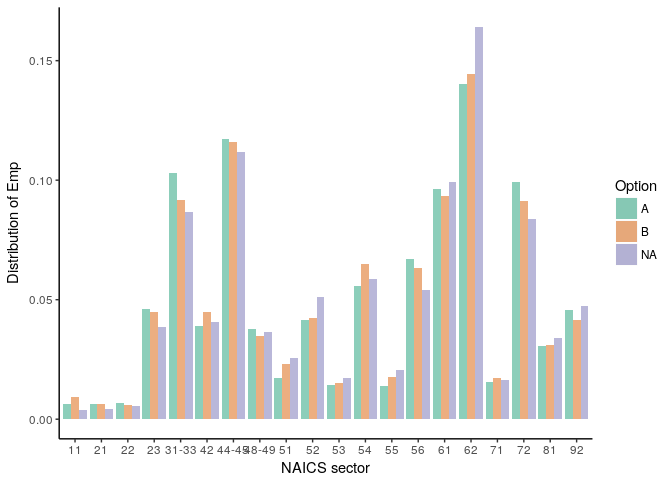
\includegraphics[height=0.9\textheight]{graph_Emp-1.png}
\end{frame}



\begin{frame}
	\frametitle{By separations}
	\centering
	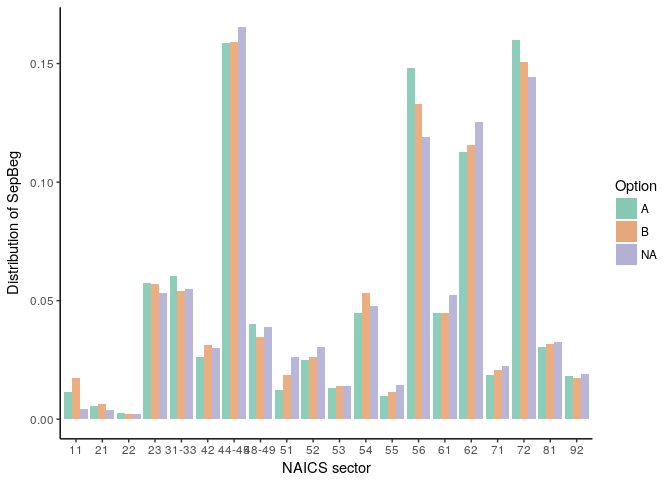
\includegraphics[height=0.9\textheight]{graph_SepBeg-1.png}
\end{frame}




\begin{frame}
\frametitle{Representativeness}
Is the sample of states representative $=$ state's choice of Option A ($M$)  correlated with any observable characteristic ($Y$):

$$p(M | Y, \theta, \psi) = p(M|\psi)$$

where $\theta$ are parameters associated with the data generating process, and $\psi$ are parameters associated with the choice of Option A. If not, then missing states are ``\ac{MCAR}''. 
\begin{block}{Generalisation}
	Replace ``Option A'' with ``is part of my research study''
\end{block}
\end{frame}


\begin{frame}
\frametitle{MCAR by employment}
\small \centering

% Table created by stargazer v.5.2 by Marek Hlavac, Harvard University. E-mail: hlavac at fas.harvard.edu
% Date and time: Wed, Sep 13, 2017 - 01:39:39 PM
\begin{tabular}{@{\extracolsep{5pt}}lc} 
\\[-1.8ex]\hline 
\hline \\[-1.8ex] 
\\[-1.8ex] & Option \\ 
\hline \\[-1.8ex] 
 Constant & 0.888$^{***}$ \\ 
  & (0.094) \\ 
  & \\ 
 Emp & 0.295$^{***}$ \\ 
  & (0.068) \\ 
  & \\ 
Akaike Inf. Crit. & 1,082.799 \\ 
\hline 
\hline \\[-1.8ex] 
\textit{Notes:} & \multicolumn{1}{r}{$^{***}$Significant at the 1 percent level.} \\ 
 & \multicolumn{1}{r}{$^{**}$Significant at the 5 percent level.} \\ 
 & \multicolumn{1}{r}{$^{*}$Significant at the 10 percent level.} \\ 
\end{tabular} 

\end{frame}


\begin{frame}
\frametitle{MCAR by employment (b)}
\small \centering

% Table created by stargazer v.5.2 by Marek Hlavac, Harvard University. E-mail: hlavac at fas.harvard.edu
% Date and time: Wed, Sep 13, 2017 - 01:39:39 PM
\begin{tabular}{@{\extracolsep{5pt}}lc} 
\\[-1.8ex]\hline 
\hline \\[-1.8ex] 
\\[-1.8ex] & Option \\ 
\hline \\[-1.8ex] 
 Constant & 0.198$^{***}$ \\ 
  & (0.076) \\ 
  & \\ 
 Emp & $-$0.124$^{***}$ \\ 
  & (0.035) \\ 
  & \\ 
Akaike Inf. Crit. & 1,400.767 \\ 
\hline 
\hline \\[-1.8ex] 
\textit{Notes:} & \multicolumn{1}{r}{$^{***}$Significant at the 1 percent level.} \\ 
 & \multicolumn{1}{r}{$^{**}$Significant at the 5 percent level.} \\ 
 & \multicolumn{1}{r}{$^{*}$Significant at the 10 percent level.} \\ 
\end{tabular} 

\end{frame}

\begin{frame}
	\frametitle{MCAR by separations}
	\small \centering
	
% Table created by stargazer v.5.2 by Marek Hlavac, Harvard University. E-mail: hlavac at fas.harvard.edu
% Date and time: Wed, Sep 13, 2017 - 01:39:41 PM
\begin{tabular}{@{\extracolsep{5pt}}lc} 
\\[-1.8ex]\hline 
\hline \\[-1.8ex] 
\\[-1.8ex] & Option \\ 
\hline \\[-1.8ex] 
 Constant & 0.979$^{***}$ \\ 
  & (0.089) \\ 
  & \\ 
 SepBeg & 0.204$^{***}$ \\ 
  & (0.058) \\ 
  & \\ 
Akaike Inf. Crit. & 1,093.073 \\ 
\hline 
\hline \\[-1.8ex] 
\textit{Notes:} & \multicolumn{1}{r}{$^{***}$Significant at the 1 percent level.} \\ 
 & \multicolumn{1}{r}{$^{**}$Significant at the 5 percent level.} \\ 
 & \multicolumn{1}{r}{$^{*}$Significant at the 10 percent level.} \\ 
\end{tabular} 

\end{frame}


\begin{frame}
	\frametitle{MCAR by both}
	\small \centering
	
% Table created by stargazer v.5.2 by Marek Hlavac, Harvard University. E-mail: hlavac at fas.harvard.edu
% Date and time: Wed, Sep 13, 2017 - 01:39:41 PM
\begin{tabular}{@{\extracolsep{5pt}}lc} 
\\[-1.8ex]\hline 
\hline \\[-1.8ex] 
\\[-1.8ex] & Option \\ 
\hline \\[-1.8ex] 
 Constant & 0.884$^{***}$ \\ 
  & (0.094) \\ 
  & \\ 
 Emp & 0.403$^{***}$ \\ 
  & (0.130) \\ 
  & \\ 
 SepBeg & $-$0.104 \\ 
  & (0.101) \\ 
  & \\ 
Akaike Inf. Crit. & 1,083.793 \\ 
\hline 
\hline \\[-1.8ex] 
\textit{Notes:} & \multicolumn{1}{r}{$^{***}$Significant at the 1 percent level.} \\ 
 & \multicolumn{1}{r}{$^{**}$Significant at the 5 percent level.} \\ 
 & \multicolumn{1}{r}{$^{*}$Significant at the 10 percent level.} \\ 
\end{tabular} 

\end{frame}

\subsection{Take-away}
\begin{frame}
	\frametitle{Representativeness}
\begin{block}{Approximately...}
  \begin{itemize}
  	\item The snapshot is \textit{approximately} representative (eye-ball test), 
  	\item ... but that statement does not hold up to an econometric test
  	\item To apply this particular criterion to your specific paper, see \textbf{\href{https://github.com/larsvilhuber/snapshot-availability}{github.com/larsvilhuber/snapshot-availability}}
  \end{itemize}
\end{block}
\end{frame}


\section{What's new}

\subsection{Overview}
\begin{frame}
\frametitle{The following components have changes}
\begin{itemize}
	\item \textbf{\ac{EHF}}: earnings at all firms for workers
	\item \textbf{\ac{ECF}}: time-varying characteristics for firms, including industry and QCEW employment
	\item \textbf{\ac{GAL}}: geo-coded addresses of firms from a variety of sources
	\item \textbf{\ac{OPM}}: earnings records for federal workers
	\item \textbf{\ac{QWI}(-SEINUNIT)}: pre-computed job market indicators (separations, job creation, etc.) at the establishment level, by worker demographics
\end{itemize}
\end{frame}


\subsection{EHF}
\begin{frame}
\frametitle{\ac{EHF}: New National Indicator of Employment}
Does a worker have covered employment in \textbf{any} state?

\begin{block}{Construction}
\small For each PIK $i$, in each EHF state file $s$, identify the  quarters $q$ in which at least \$1 was earned in any job $j$:
$$
\forall i, \forall q, \forall s: pos\_earn_{isq} = 1 \text{\ if} \left ( \sum_{\substack{j: J(i,q)=1 \\ \land J(s,q) = 1}} earn_{ijq}  \right ) \geq 1
$$
where $J(i,q)$ indicates that $i$ worked for $j$ in $q$ and $J(s,q)$ indicates that $j$ is located in $s$ in $q$. 
Count the \textbf{number} of states (not jobs):
$$
\forall i, \forall q: pos\_earn_{iq} = \sum_{s} pos\_earn_{isq}
$$
\end{block}
\end{frame}
\note{

 This file is useful for researchers who only have access to a subset of the national data, but need to identify labor force status in other states, for instance to do a Heckman-style correction. This file is designed to permit such analyses.
}

\begin{frame}
\frametitle{\ac{EHF}: New National Indicator of Employment}
The file is not subject to state-specific restrictions, and is automatically added to any project requesting LEHD data.
\end{frame}

\begin{frame}
\frametitle{EHF availability metadata}

Temporal availability of states  (\texttt{ehf\_all\_availability}), so that users can control for the at-risk states at each point in time 
\end{frame}
\note{
Note: Researchers often request, or otherwise re-compute information for when each state EHF file starts and ends. 
}

%\frametitle{File format of EHF-PHF}
%The EHF-PHF, a wide version of the regular EHF (one observation for job, rather than one observation per job-year), is often used by researchers since it provides convenient access to all earnings on a given job. No additional information is available on the EHF-PHF, only the organization of the data is different. In this snapshot, in order to deduplicate data and conserve scarce disk space, this file has been converted from a physical file to a SAS view. Users should notice no difference in file access speed or use of the file. Users should read the SAS documentation to learn more about SAS views.

\subsection{ECF}

\begin{frame}[fragile]
	\frametitle{Restructured \ac{ECF}}
\begin{block}{Compatibility}
\begin{itemize}
	\item Not completely backward compatible: some variables   changed names / no longer produced 
	\item \textbf{No changes} have been made to T26 variables $\rightarrow$ no change in permissions required
\end{itemize}
\end{block}

\begin{block}{NAICS and SIC}
	\begin{itemize}
	\item NAICS2012 codings are now available, in addition to other NAICS vintages
	\item SIC1987-based codings  still available, consistently named 
	\end{itemize}
\end{block}
\end{frame}

\note{The \ac{ECF} has been restructured. The fundamental variables typically used by  researchers remain available, but some variables  have changed names or are no longer produced by the production system. Tables provide information on these changes.}

\subsection{GAL}

\begin{frame}
	\frametitle{\ac{GAL} restructured}
\begin{itemize}
	\item Completely restructured in production system 
	\item An attempt was made to maintain backward compatibility, but \textbf{not all changes} could be reasonably mapped. 
	\item \textbf{Crosswalks} to all input sources have been \textbf{re-introduced.}
\end{itemize}
\end{frame}

\subsection{OPM}

\begin{frame}
	\frametitle{\acf{OPM}}
	\begin{itemize}
		\item 	\ac{OPM} data on Federal workers  have been collected under a \textbf{single directory}. RDC users should be able to access these files by requesting a ``OPM'' dataset. 
		\item Access to the OPM data \textbf{do not require state} permissions. 
	\end{itemize}
\end{frame}


\subsection{QWI}

\begin{frame}
\frametitle{\acf{QWI} SEINUNIT}
\begin{block}{Renamed and dropped variables}
	\begin{itemize}
		\item In line with changed publication of QWI (\href{https://lehd.ces.census.gov/doc/Memo_changes_to_QWI.pdf}{lehd.ces.census.gov/doc/Memo\_changes\_to\_QWI.pdf}), several variables are no longer present, or have been renamed. \item In general, names are consistent with the "Alternate names" in  (\href{https://lehd.ces.census.gov/data/schema/V4.0.1/lehd_public_use_schema.html}{LEHD Schema V4.0.1})
	    \item Coding for race and ethnicity has changed, this affects the \textbf{naming} of variables.
\end{itemize}
\end{block}
\end{frame}

\begin{frame}
	\frametitle{QWI SEINUNIT}
The following variables are no longer available:
\begin{itemize}
	\item All variables related to \emph{changes in total earnings} (starting with {\tt dW})
	\item All variables that are rates (ending in {\tt R})
	\item All variables related to periods of non-employment preceding or following a transition (starting with {\tt N})
	\item Certain average earnings variables ({\tt WCA, WCS, WA, WS})
	\item Certain variables relating to continuous quarter hiring ({\tt CH}, {\tt CR})
	\item The variable {\tt FSnx} (Full-quarter separations in the \textbf{next quarter})
	\item The variable {\tt W2} (average earnings for \textbf{end-of-quarter} employment), replaced by {\tt W2B} (average earnings for \textbf{beginning-of-quarter} employment)
\end{itemize}
\end{frame}
\note{
The following variables have been renamed:
\begin{itemize}
	\item The name of the SIC variable has changed from {\tt ES\_SIC} to {\tt SIC1987FNL }
	\item The name of the NAICS variable has changed from {\tt ES\_NAICS\_FNL2007} to {\tt NAICS2012fnl} and reflects NAICS 2012 coding.
	\item The name of {\tt H3} (New Hires into Full-Quarter Employment) has been changed to {\tt FH	} for consistency with the public-use variables.
	
	\item Earnings-related variables have been made consistent with the public-use variables
	\begin{tabular}{lll}
		Public-use name & Internal name & Label\\
		\hline
		ZW3 &	W3&	Average Monthly Earnings (Full-Quarter Employment)\\
		ZW1	&  W2B&	Average Monthly Earnings (Beginning-of-Quarter Employment)\\
		ZWFA&  WFA&	Average Monthly Earnings (All Hires into Full-Quarter Employment)\\
		ZWFH&  WH3&	Average Monthly Earnings (New Hires into Full-Quarter Employment)\\
		ZWFS&  WFS&	Average Monthly Earnings (Flows out of Full-Quarter Employment)\\
	\end{tabular}
\end{itemize}
}	






\section{Availability}
\begin{frame}
\frametitle{When is it available to researchers}
\begin{block}{Integrated Research Environment (IRE)}
The S2014 Snapshot will become available when the IRE is made accessible to FSRDC researchers.
\end{block}
\end{frame}

 
\begin{frame}[fragile]  % notice the fragile option, since the body
			% contains a verbatim command
\vspace{1in}
\centerline{The End}
\vspace{3in}
\tiny

\end{frame}
% End of slides


\begin{frame}[shrink]
\renewcommand*{\bibfont}{\tiny}
\begin{block}{References}
\printbibliography[heading=none]
\end{block}
\end{frame}


\end{document} 
